\section{Điểm nổi bật và đóng góp của dự án}

    \subsection{Kết nối thị giác máy tính với dự báo chuỗi thời gian}
    Dự án không dừng ở hình có bounding box. Số đếm được chuyển thành một chuỗi đo có timestamp, tổng hợp theo phút, dùng cùng định nghĩa đặc trưng khi train và chạy trực tiếp, rồi biến thành đường dự báo và ETA. Sự liên kết này là đóng góp ứng dụng rõ ràng: mỗi bước có đầu vào và đầu ra có thể kiểm tra, thay vì chỉ trình diễn một mô hình riêng lẻ.

    \begin{figure}[htbp]
        \centering
        % 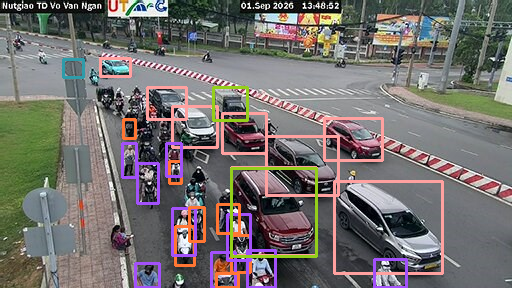
\includegraphics[width=0.85\textwidth]{runs/supervision_test9.png}
        \caption{Kết quả lưu từ thử nghiệm Supervision tại \texttt{runs/supervision\_test9.png}, minh họa nhiều phương tiện nhỏ và che khuất trong cảnh nút giao. Script thử nghiệm sử dụng lát $512 \times 512$; ảnh không phải bảng đo precision/recall và không chứng minh ưu thế định lượng so với lát $256 \times 256$.}
        \label{fig:supervision_test}
    \end{figure}

    \subsection{Phân biệt dữ liệu thật, tham chiếu và dữ liệu mất}
    Khởi động ứng dụng tạo ra một vấn đề thực tế: model cần 61 điểm phút, nhưng người dùng muốn nhìn thấy thông tin ngay. Dự án giải quyết bằng tham chiếu học từ data1, đánh dấu riêng các phút tham chiếu và dùng một nhánh tạm thời. Khi quan sát thật tích lũy, chúng thay thế tham chiếu; khi đủ điều kiện mới chuyển sang model.

    Điểm đáng chú ý là lịch sử tham chiếu không được đưa vào estimator như dữ liệu đo thật, và mất camera sau khởi động không bị che bằng một đường nội suy. Cách xử lý này giữ được ý nghĩa của phép đo và trạng thái chất lượng dữ liệu.

    \subsection{Giữ danh tính nguồn dự báo khi người dùng đổi camera}
    Giao diện cho phép chọn camera để xem, nhưng nguồn dự báo luôn là Camera 1. \texttt{CameraWorker} phát số đếm từ camera dự báo cố định; \texttt{ForecastWorker} loại mẫu có tên camera khác. Nhờ đó thao tác đổi góc xem không làm lịch sử chuỗi thời gian bị trộn giữa hai vị trí.

    Tính độc lập về nguồn không đồng nghĩa độc lập về tài nguyên: việc lấy ảnh và nhận diện camera đang xem thêm vẫn nằm trong vòng worker, có thể làm chu kỳ Camera 1 dài hơn. Chưa có số đo latency để định lượng ảnh hưởng.

    \subsection{Xử lý bất đồng bộ và lưu bằng chứng trước khi biết tương lai}
    Thu ảnh/YOLO và dự báo được đưa ra khỏi luồng giao diện. Model chỉ tải một lần; biểu đồ tái sử dụng Figure và các đối tượng vẽ khi cập nhật. Đây là lựa chọn nhằm giữ UI đáp ứng mà không cần huấn luyện lại hoặc dựng lại toàn bộ biểu đồ mỗi lần có dữ liệu.

    SQLite lưu timestamp quan sát, origin dự báo, thời điểm phát, các giá trị dự báo thô/đã làm mượt, model ID và phương pháp. Script \texttt{evaluate\_live\_forecasts.py} chỉ lấy lần phát đầu tiên của mỗi origin, loại dự báo phát quá muộn và chỉ chấm khi đủ dữ liệu tương lai với độ phủ mẫu yêu cầu. Nhờ vậy việc đánh giá không chọn lại một phiên bản dự báo thuận lợi sau khi đã biết kết quả.

    Lịch sử được khôi phục khi ứng dụng mở lại, nhưng khoảng thời gian ứng dụng tắt vẫn là khoảng thiếu. Collector ghi theo lô ngắn cũng giảm nguy cơ mất toàn bộ đợt thu; việc dừng cưỡng bức vẫn có thể làm mất lô chưa ghi cuối cùng.

    \subsection{Kiểm tra tính tương thích và bảo vệ model đang dùng}
    Bundle dự báo chứa danh sách và thứ tự đặc trưng, horizon, history window, target mode, đường tham chiếu, metrics và thông tin phiên bản môi trường. \texttt{validate\_bundle()} kiểm tra cấu trúc quan trọng trước khi suy luận, bao gồm đủ 60 estimator và đúng thứ tự cột.

    Huấn luyện mới không tự ghi đè artifact đang tồn tại: script chuyển sang tên candidate, lưu model rồi tải lại để so sánh một dự báo với kết quả trước khi lưu. Thiết kế này tạo cơ sở cho việc kiểm tra ứng viên trước khi thay model đang vận hành. Tuy nhiên, script chưa có cổng tự động từ chối triển khai theo toàn bộ tiêu chí cảnh báo; việc lưu thành công không chứng minh model mới tốt hơn.

    \subsection{Kiểm thử hướng vào lỗi có ý nghĩa}
    Các tệp test hiện có bao phủ những tình huống như feature không sử dụng tương lai, đúng thứ tự lag 60, lệch schema, thiếu model, timestamp dự báo, quy tắc 3/5, mất mẫu, phút thưa, đổi camera, khôi phục SQLite, giữ phiên bản forecast và ghi CSV khi có lỗi nhận diện.

    Báo cáo này đọc các kiểm thử để xác định ý đồ và phạm vi bảo vệ của hệ thống, không báo chúng là một lượt test mới đã chạy. Kiểm thử logic hoặc ảnh UI chỉ xác nhận từng phần hành vi; độ chính xác giao thông trực tiếp vẫn cần quan sát tương lai có nhãn và nhật ký tương ứng.

    Những điểm nổi bật trên là đóng góp kỹ thuật trong phạm vi dự án. Tài liệu chưa đưa ra bằng chứng về một thuật toán học máy mới hoặc so sánh học thuật để khẳng định tính mới ở cấp nghiên cứu phương pháp.

